\chapter{Architecture du projet}

\section{L'image du mode recovery}

\subsection{L'image de base}
Le mode Recovery se base sur le kernel Linux 2.6.35.3 qui est contenu dans une ROM interne à la liseuse (il est donc inaccessible). Le système de fichier est présent dans un fichier de type image contenu lui sur la carte SD. Ce fichier peut être modifié depuis un PC en montant l'image.

L'image fournie par défaut pour le mode Recovery, contient : 
\begin{itemize}
	\item un exécutable Busybox \\
		qui permet l'accès aux commandes usuelles Linux dans les systèmes embarqués
	\item un serveur DHCP
	\item un démon telnet
	%peut etre a mettre dans la partie du rapport intermediaire
	\item un accès au port USB en mode série (via le module g_serial)
\end{itemize}


Le système de fichier du mode Recovery est en lecture seule, seuls les dossiers suivant sont accessibles en lecture / écriture : 
\begin{itemize}
	\item /etc
	\item /initrd/mnt/sd
	\item /tmp
\end{itemize}

Pour modifier le système de fichier racine il faut passer par un PC hôte.

\subsection{L'image finale}

L'image finale ajoute les fonctionnalités suivante à l'image : 
	\begin{itemize}
		\item un accès au port USB par connexion Ethernet
		\item le support du protocole SSH
		\item la librairie DirectFB
	\end{itemize}

On a désactivé le serveur DHCP de la liseuse : \\
		il est peu utile d'avoir un support DHCP alors que le PC hôte et la liseuse 
		ont un réseau pour eux seuls.
		%peut etre rajouté le fait qu'il sont en plus défini statiquement ??

~\\

L'émulation d'un lien Ethernet sur le port USB de la liseuse se fait via le module g_ether.
%a verifier si c'est pas déjà dis avant
Ce module est situé comme les autres modules dans :
	\begin{lstlisting}
	/lib/modules/2.6.35.3/kernel/drivers/usb/gadget
	\end{lstlisting}

Le support du protocole SSH se fait via l'exécutable Dropbear situé dans : 
	\begin{lstlisting}
	/bin
	\end{lstlisting}

Les fichiers concernant la librairie DirectFB se situe dans le dossier /usr/local/lib.
Pour pouvoir lancer une exécutable utilisant DirectFB il faut vérifier que ce dossier soit bien inclus dans la variable d'environnement LD_LIBRARY_PATH.
\section{La mise en place de l'affichage}
%architecture pour affichage via directfb

L'affichage de la liseuse se fait grâce aux modules suivant : 
\begin{itemize}
	\item le driver mxc_epdc
	\item DirectFB
\end{itemize}~\\

Le driver se charge de faire les optimisations pour pallier au problème de réactivité de l'écran (via les tables LuT notamment), ainsi que l'application des waveforms pour l'affichage sur l'écran.\\
Le driver fournit des ioctl pour permettre l'exécution des fonctionnalités du driver depuis l'espace utilisateur.~\\~\\
%verifier si c'est pas deja dis plus tot dans le rapport
DirectFB implémente des primitives graphiques, comme le traçage de ligne. Ces dernières permettent de faire une abstraction sur le format du framebuffer.

Voici un schéma modulaire de l'application utilisant DirectFB : 

\begin{figure}[h!]
	\begin{center}	
		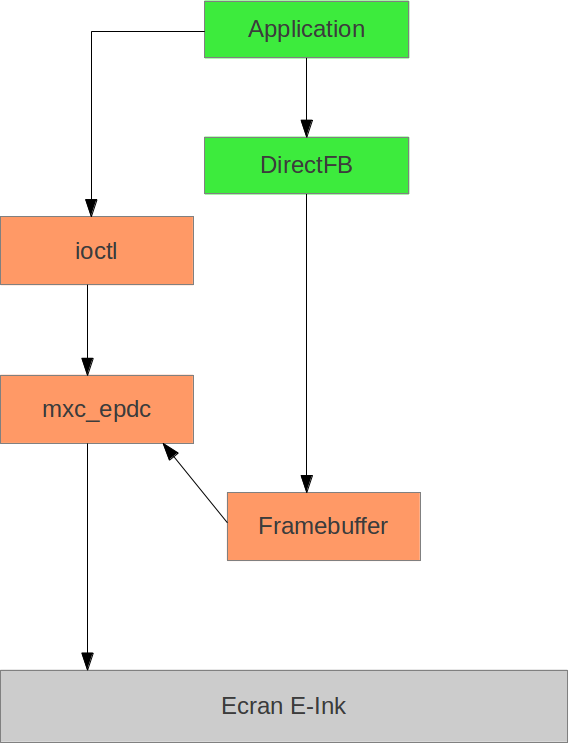
\includegraphics[scale=0.5]{schema_direct_fb.png}
		\caption{Architecture modulaire de l'application}
	\end{center}
\end{figure}

Dans l'état d'avancement actuel du projet, le programme met à jour le framebuffer via DirectFB et fait un appel ioctl au driver qui actualise l'écran en fonction du buffer. 
% application => directfb => framebuffer 				=> affichage
%						 => ioctl 	=> driver epdc   ||


%explication du fonctionnement 

% description de chaque module 
% directfb : abstraction du driver d'affichage
% ioctl : appel de la maj driver
%
%framebuffer